\chapter{Analisis Data Fisik}

\section{Membuat Data Universal}
Dalam pembuatan data universal ini kita menuliskan semua atribut universal yang dimiliki oleh setiap berkas, sebagai berikut :
\begin{itemize}

	\item Kartu Keluarga\\
		Nomor Induk Kartu Keluarga\\
		Nomor Kartu Keluarga\\
		Nama Kepala Keluarga\\
		Alamat\\
		RT/RW\\
		Desa/Kelurahan\\
		Kecamatan\\
		Kabupaten/Kota\\
		Kode Pos\\
		Provinsi\\
		Nama Lengkap\\
		NIK\\
		Jenis Kelamin\\
		Tempat Lahir\\
		Tanggal Lahir\\
		Agama\\
		Pendidikan\\
		Jenis Pekerjaan\\
		Status Perkawinan\\
		Hubungan Keluarga\\
		Kewarganegaraan\\
		Nomor Passport\\
		Nomor KITAS/KITAP\\
		Nama Ayah\\
		Nama Ibu\\
		Jumlah Anggota\\
		Tanggal, Bulan, dan Tahun terbit KK\\
		Tanda Tangan\\
		Nomor Induk Pejabat\\
		Nama Pejabat

	\item Akta Kelahiran\\
		Nomor Akta\\
		Kode CSL\\
		Dari Daftar\\
		Nomor STBLD\\
		Tanggal Kelahiran\\
		Bulan Kelahiran\\
		Tahun Kelahiran\\
		Jenis Kelamin\\
		Nama Kelahiran\\
		Urutan Anak\\
		Tanggal Bulan Tahun Surat Keluar\\
		Nama Pejabat\\
		Tanda Tangan Pejabat\\
		Nama Ayah\\
		Nama Ibu\\
		Kota dan Hari Kelahiran
		
	\item Formulir F-1.21\\
		Pemerintah Provinsi\\
		Pemerintah Kabupaten/Kota\\
		Kecamatan\\
		Kelurahan/Desa\\
		Jenis Permohonan KTP\\
		Nama Lengkap\\
		No. KK\\
		NIK\\
		Alamat\\
		RT\\
		RW\\
		Kode Pos\\
		Pas Foto 2x3\\
		Cap Jempol\\
		Tanda Tangan\\
		Kota\\
		Tanggal, Bulan, Tahun Pengisian Formulir\\
		NIP\\
		Nama Pejabat

	\item Surat Pengantar RT dan RW\\
		Nomor Surat Pengantar\\
		Nama RT\\
		Jabatan\\
		Alamat RT\\
		Nama Lengkap Pemohon\\
		Jenis Kelamin\\
		Agama\\
		Status\\
		NIK\\
		Tempat dan Tanggal Lahir\\
		Pekerjaan\\
		Alamat\\
		Keperluan\\
		Keterangan Lain Lain\\
		Berlaku Mulai\\
		Tanda Tangan\\
		Tanggal Bulan Tahun Pembuatan Surat

	\item e-KTP\\
		Provinsi\\
		Kabupaten\\
		NIK\\
		Nama\\
		Tempat/Tanggal Lahir\\
		Jenis Kelamin\\
		Golongan Darah\\
		Alamat\\
		RT/RW\\
		Kelurahan/Desa\\
		Kecamatan\\
		Agama\\
		Status Perkawinan\\
		Pekerjaan\\
		Kewarganegaraan\\
		Berlaku Hingga\\
		Foto\\
		Kota terbit\\
		Tanggal Bulan Tahun diterbitkannya e-KTP\\
		Tanda Tangan\\

\end{itemize}

Kami berdiskusi bahwa cara kita menganalisa data tersebut agar tidak terjadinya redudansi adalah dengan cara melihat kesamaan data dari beberapa berkas yang tersedia, contohnya adalah Nama. Nama sangatlah krusial dalam database, maka dari itu agar tidak terjadinya redudansi kita semu sepakat bahwa atribut nama hanya boleh berada di 1 tabel dan ini berlaku ke semua atribut yang berada dalam berkas tersebut, kecuali tanggal bulan dan tahun karena data tersebut saat dipergunakan dapat berubah-ubah jadi menurut kami tidak masalah seperti tanggal, bulan, dan tahun kelahiran dengan tanggal, bulan, dan tahun terbitnya e-KTP. Jadi kami menganalisa ke atribut yang memang sangat krusial terjadinya redudansi data. Setelah kita menyatukan semua atribut dan kami analisa juga atribut tersebut pertama kali berada dimana maka atribut tersebut berada di tabel yang seharusnya berada, contoh Nama. Nama seseorang menurut analisa kami itu sangat kuat/erat kaitannya dengan akta kelahiran karena berkas seseorang pertama kali yang resmi adalah akta kelahiran, dan menurut analisa kami untuk terjadinya ada nik yang berada di kartu keluarga itu berasal dari akta kelahiran, maka kami menyimpulkan bahwa nama seseorang itu berada di tabel akta kelahiran.

Setelah semua data kita analisis maka ini hasil tabel yg sudah kita buat :

\begin{figure}[H]
	\centering
	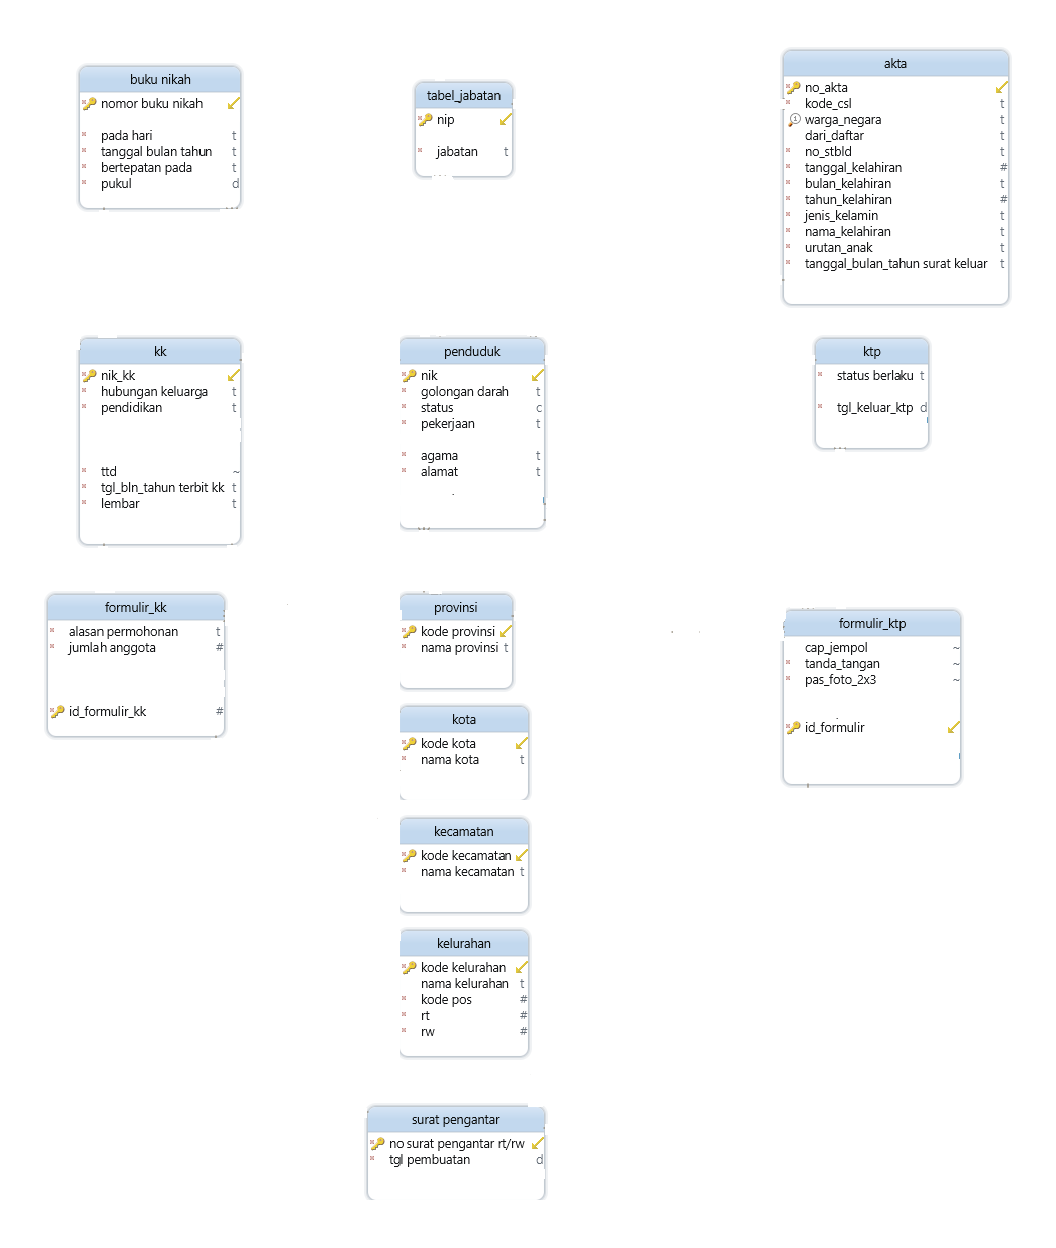
\includegraphics[width=12cm]{figures/0002t.png}
	\caption{Tabel Database.}	
\end{figure}

Kita juga menambahkan beberapa atribut untuk dijadikan atribut Primary Key (PK) seperti id formulir menurut analisa kami, petugas memberikan id formulir yang saat pemohon/warga menyerahkan berkas-berkasnya.